\documentclass{scrartcl}
\usepackage[T1]{fontenc}
\usepackage[ngerman]{babel}
\usepackage{graphicx}
\usepackage{subcaption}
\begin{document}
\section{Zwei Bildansichten}
\begin{figure}[htbp]
  \centering
  \begin{subfigure}{.47\linewidth}
    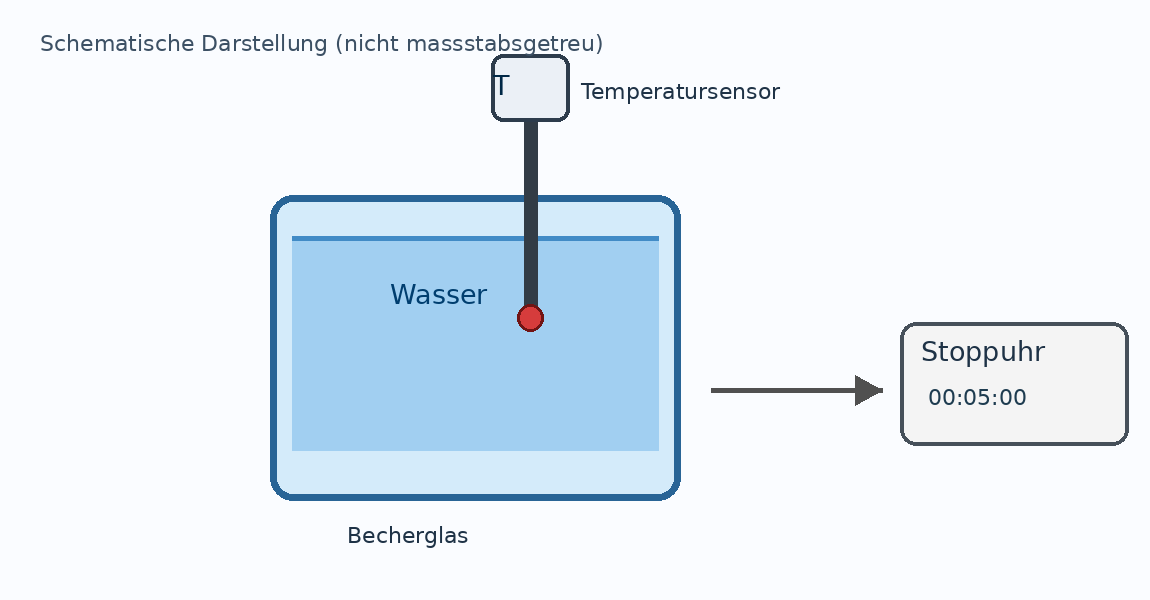
\includegraphics[width=\linewidth]{bilder/messaufbau.png}
    \caption{Ansicht A}\label{fig:ansicht-a}
  \end{subfigure}\hfill
  \begin{subfigure}{.47\linewidth}
    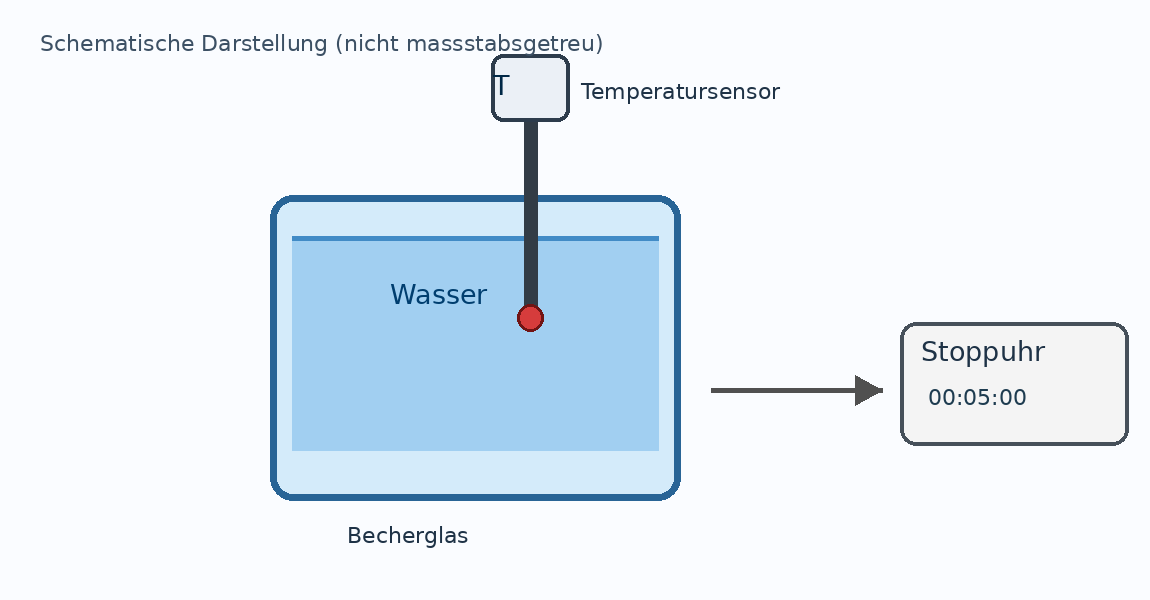
\includegraphics[width=\linewidth]{bilder/messaufbau.png}
    \caption{Ansicht B}\label{fig:ansicht-b}
  \end{subfigure}
  \caption{Vergleich zweier Ansichten}
\end{figure}
\end{document}
